\documentclass[11pt,a4paper]{article}

% ---------------------------------------------------------------
% Paquetes
% ---------------------------------------------------------------
\usepackage[utf8]{inputenc}
\usepackage[T1]{fontenc}
\usepackage[spanish,es-tabla]{babel}
\usepackage{lmodern}
\usepackage[margin=2.3cm]{geometry}
\usepackage{graphicx}
\usepackage{booktabs}
\usepackage{caption}
\usepackage{float}
\usepackage{xcolor}
\usepackage[hidelinks]{hyperref}
\usepackage{parskip}

\captionsetup{font=small,labelfont=bf}
\setlength{\parskip}{0.45em}

% ---------------------------------------------------------------
% Portada
% ---------------------------------------------------------------
\begin{document}

\begin{titlepage}
\centering
{\large Universidad de Buenos Aires · Facultad de Ciencias Económicas\par}
{\large Tecnicatura Universitaria en Gestión y Análisis de Datos en Organizaciones\par}
\vspace{0.6cm}
{\large Laboratorio de Métodos Cuantitativos · 2.º cuatrimestre 2026\par}
\vspace{3cm}
{\LARGE\bfseries Delito en el AMBA:\par}
\vspace{0.3cm}
{\Large tipo y frecuencia de los delitos denunciados según las condiciones socioeconómicas y territoriales (2017--2025)\par}
\vspace{2.5cm}
{\large\bfseries Integrantes\par}
\vspace{0.4cm}
\begin{tabular}{lll}
\toprule
Nombre & Registro & Usuario de GitHub \\
\midrule
Chietino Luna, Micaela & 921785 & @mchietino \\
Iandoli, Franco & 921507 & @Franco-Iandoli \\
Ortiz, Naiara & 921844 & @naiaraortizrodriguez \\
Peralta, Santiago & 921431 & @SantiagoNPeralta \\
Turrillo, Bruno & 921414 & @bauhaushm \\
\bottomrule
\end{tabular}
\vfill
{Repositorio: \url{https://github.com/bauhaushm/TP-Delito_en_AMBA}\par}
\vspace{0.3cm}
{Noviembre de 2026\par}
\end{titlepage}

% ---------------------------------------------------------------
% 1. Resumen
% ---------------------------------------------------------------
\section*{Resumen}
Este trabajo compara los patrones delictivos del Área Metropolitana de Buenos Aires (AMBA) entre 2017 y 2025 y analiza cómo varían el tipo y la frecuencia de los delitos según las condiciones socioeconómicas y territoriales de las comunas porteñas. Se utilizaron datos del Sistema Nacional de Información Criminal (SNIC), la Encuesta Anual de Hogares (EAH), el Censo 2022, el registro de barrios populares y el relevamiento de usos del suelo, procesados en Python. Los resultados muestran que la tasa de delitos de CABA duplica la del Conurbano, aunque este registra más hechos en total. Dentro de la Ciudad, las condiciones de vida no explican cuánto delito se registra en cada comuna, sino qué tipo predomina: los robos y hurtos se concentran en las comunas con mayor actividad comercial, mientras que los delitos violentos tienen mayor peso en las comunas más vulnerables del sur.

% ---------------------------------------------------------------
% 2. Introducción
% ---------------------------------------------------------------
\section{Introducción}
El AMBA concentra más de un tercio de la población del país y una parte importante de los delitos registrados. Conocer qué tipo de delito predomina en cada territorio, y cómo se relaciona con las condiciones de vida, permite pensar políticas de seguridad diferenciadas: no requiere la misma respuesta una zona con muchos robos asociados al comercio que otra donde pesa más la violencia interpersonal en contextos de vulnerabilidad.

La fuente principal es la base \textit{SNIC -- Departamentos. Anual} del Ministerio de Seguridad de la Nación, que informa la cantidad de hechos denunciados y su tasa cada 100.000 habitantes por tipo de delito, departamento y año. La pregunta que guía el trabajo es:

\begin{quote}
\textit{¿Cómo se comparan los patrones delictivos entre los partidos del AMBA, y de qué manera varían el tipo y la frecuencia de los delitos denunciados según las condiciones socioeconómicas y habitacionales al interior de las comunas porteñas?}
\end{quote}

Para la segunda parte de la pregunta se plantearon tres hipótesis: (i) de \textbf{oportunidad}, según la cual los delitos contra la propiedad se concentran en las comunas con mayor actividad comercial y circulación de personas; (ii) de \textbf{vulnerabilidad}, según la cual los delitos violentos tienen mayor peso en las comunas con peores condiciones sociales; y (iii) de \textbf{deterioro}, según la cual las comunas con más locales vacíos presentan mayor presencia de violencia.

% ---------------------------------------------------------------
% 3. Datos y metodología
% ---------------------------------------------------------------
\section{Datos y metodología}
La base del SNIC se recortó a las 15 comunas de CABA y los 24 partidos del Conurbano para el período 2017--2025 (21.345 registros y 6 variables: año, provincia, departamento, tipo de delito, cantidad de hechos y tasa). Se aplicaron dos exclusiones principales. Primero, se eliminaron los registros con ``Departamento sin determinar'', que concentraban todos los valores nulos de la tasa y representan el 7,08\,\% de los hechos de CABA, por lo que las cifras de la Ciudad están levemente subestimadas. Segundo, se conservaron solo los 56 tipos de delito presentes en todos los años, ya que los 10 incorporados en 2023 habrían generado un salto artificial en la serie (3,6\,\% de los hechos). La base final tiene 19.641 registros.

Entre las transformaciones se creó la variable \texttt{zona} (CABA o Conurbano), se calculó la tasa total de cada territorio sumando las tasas de los distintos tipos de delito y se agruparon los delitos en dos categorías: \textbf{contra la propiedad} (robos, hurtos y sus tentativas) y \textbf{violentos} (lesiones dolosas, amenazas y homicidios dolosos).

Para las comunas de CABA se incorporaron cuatro fuentes complementarias: la EAH del IDECBA (ingreso per cápita familiar relativo al promedio de la Ciudad, desocupación y hacinamiento), el Censo 2022 (cobertura de salud, nivel educativo, vivienda y tenencia), el registro de barrios populares y el relevamiento de usos del suelo 2022--2024 (locales comerciales y proporción de locales vacíos). Las comunas se agruparon en tres zonas: Norte (2, 11, 12, 13 y 14), Centro (1, 3, 5, 6, 7, 10 y 15) y Sur (4, 8 y 9). Todas las fuentes se unieron por número de comuna. El análisis se realizó en Google Colab con \texttt{pandas}, \texttt{matplotlib} y \texttt{seaborn}.

% ---------------------------------------------------------------
% 4. Resultados
% ---------------------------------------------------------------
\section{Resultados}

\subsection{CABA y el Conurbano}
El Conurbano registra entre 1,3 y 2,0 veces más hechos que CABA en todos los años, en parte por su mayor población. Al considerar la tasa, la relación se invierte: el promedio anual es de unos 5.620 hechos cada 100.000 habitantes en las comunas porteñas y de unos 2.720 en los partidos del Conurbano. La diferencia es sistemática, ya que la comuna con menor tasa (Comuna 6, 4.012) supera al partido con la tasa más alta (Morón, 3.727). Ambas zonas alcanzaron su máximo en 2019 y cayeron en 2020, año de las restricciones por la pandemia (Figura~\ref{fig:serie}). Entre 2017 y 2025 la tasa de CABA se mantuvo estable ($-0{,}4$\,\%), mientras que la del Conurbano creció un 17,9\,\%, por lo que la brecha se redujo.

\begin{figure}[H]
\centering
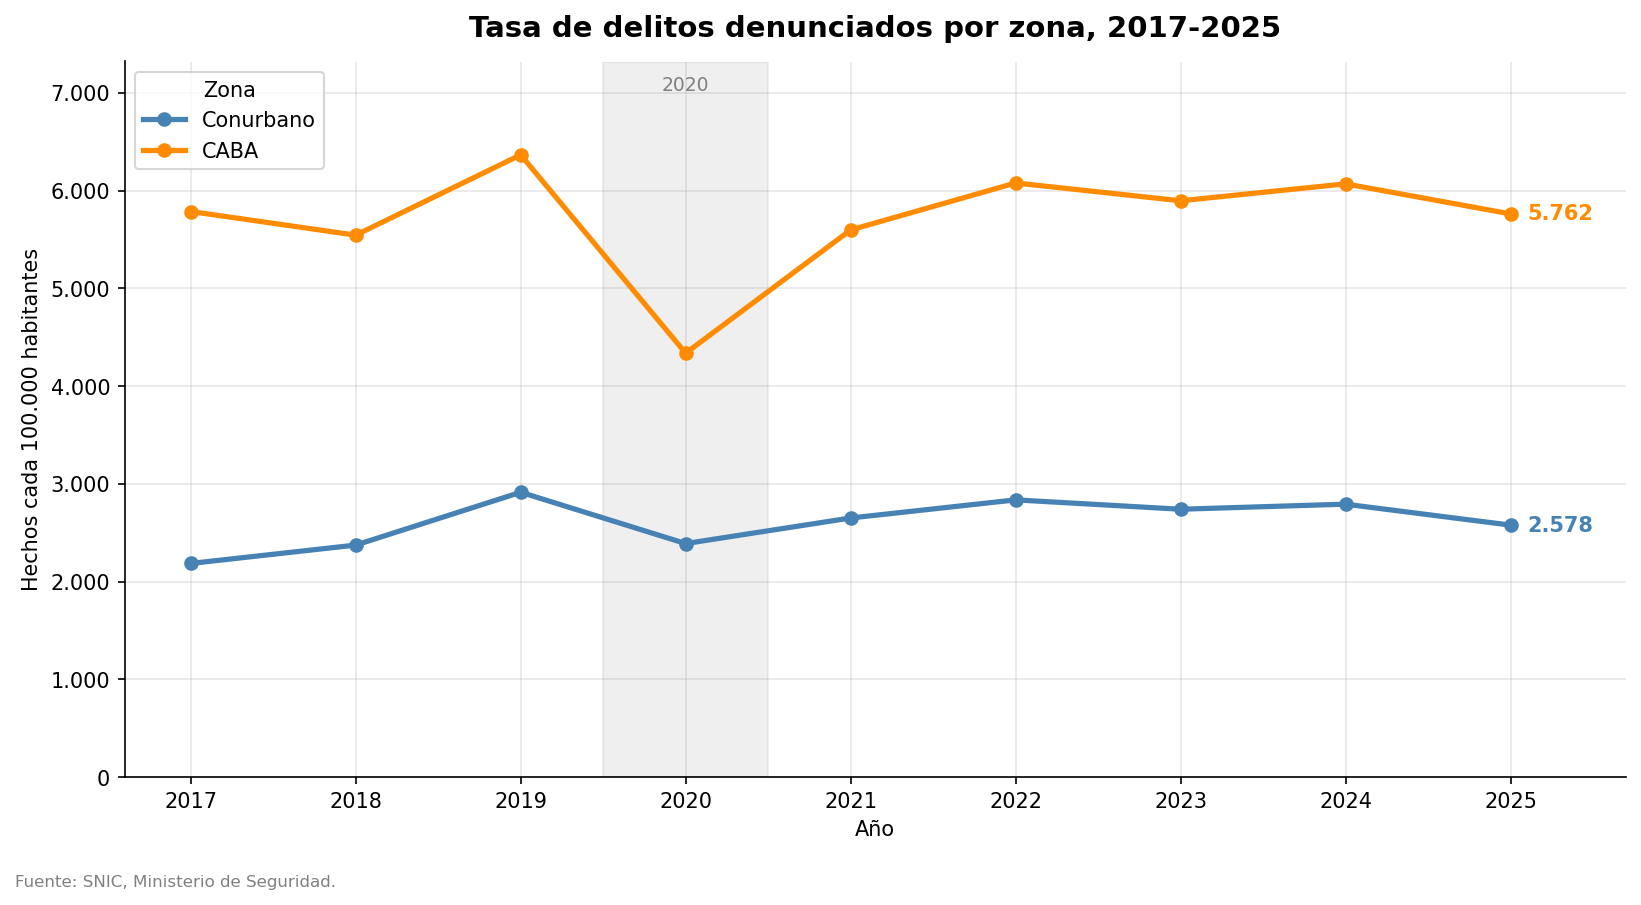
\includegraphics[width=0.78\textwidth]{tasa_total_zonas.png}
\caption{Tasa total de delitos cada 100.000 habitantes por zona, 2017--2025. Fuente: SNIC.}
\label{fig:serie}
\end{figure}

La composición también difiere (Figura~\ref{fig:tipos}). Robos y hurtos suman el 59\,\% de los hechos de CABA y el 43,7\,\% de los del Conurbano, donde pesan más las amenazas (13,5\,\% frente a 5,2\,\%) y las lesiones dolosas (10,9\,\% frente a 6,4\,\%). Mientras en CABA la evolución de la tasa depende de los delitos contra la propiedad, en el Conurbano estos se mantienen por debajo de 2019 y crecen los delitos contra las personas.

\begin{figure}[H]
\centering
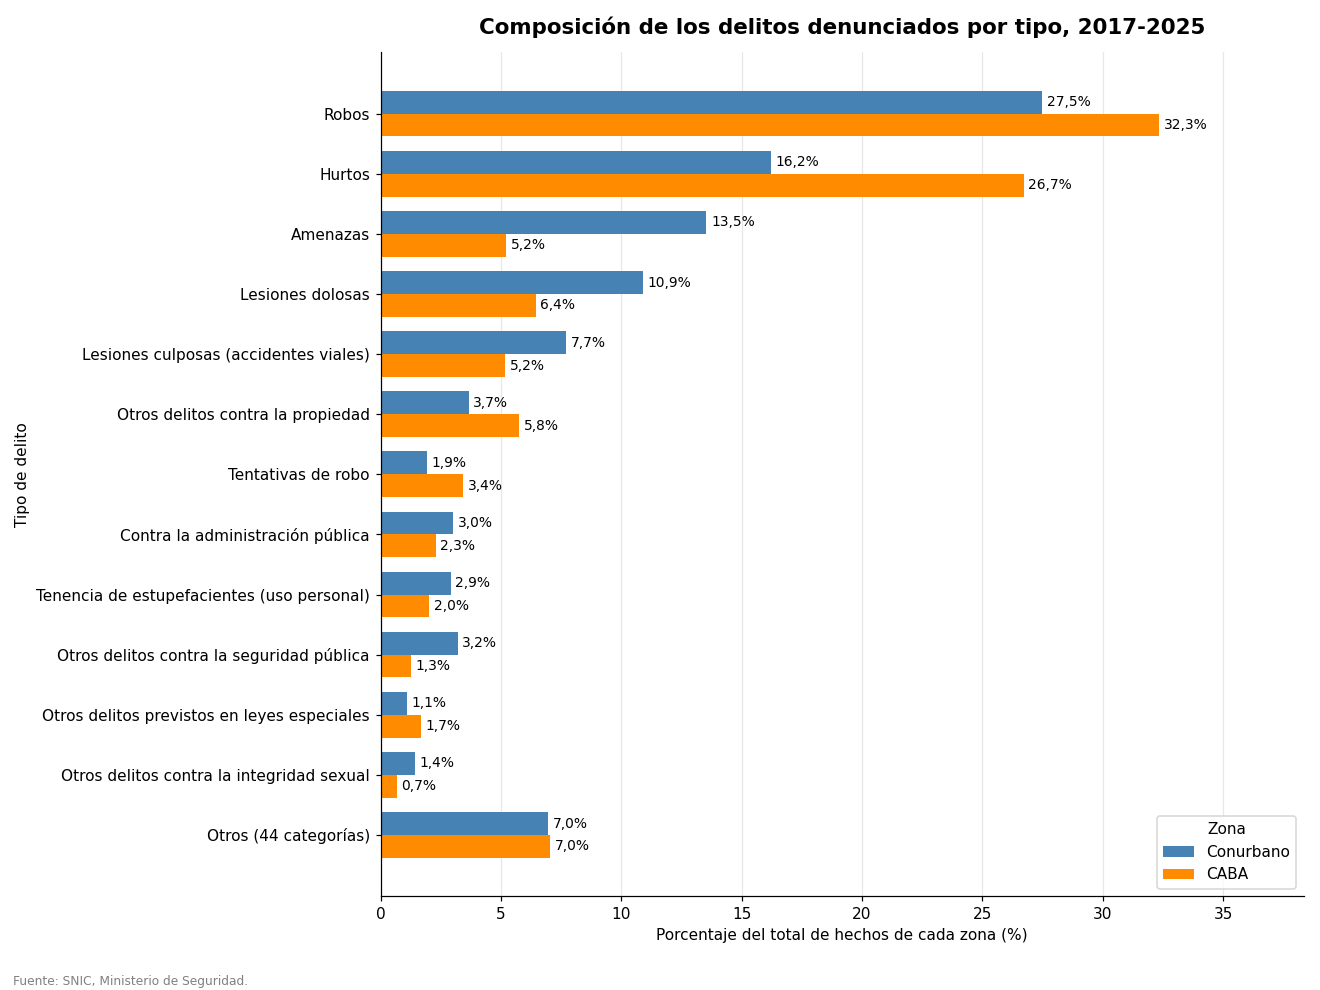
\includegraphics[width=0.62\textwidth]{tipos_delito.png}
\caption{Composición de los delitos por tipo en cada zona, 2017--2025 (\% del total de hechos). Fuente: SNIC.}
\label{fig:tipos}
\end{figure}

\subsection{Delito y condiciones socioeconómicas en las comunas de CABA}
Dentro de la Ciudad, la tasa varía fuertemente: la Comuna 1 (10.381) casi triplica a la Comuna 6 (4.012), y las comunas con mayores tasas (1, 3, 4, 14 y 9) pertenecen a las tres zonas. La relación entre la tasa de delito y el ingreso es débil (Figura~\ref{fig:ingreso}): la Comuna 1, con ingresos cercanos al promedio, tiene la tasa más alta; la Comuna 8, la de menores ingresos, queda por debajo del promedio; y la Comuna 14, la de mayores ingresos, lo supera.

\begin{figure}[H]
\centering
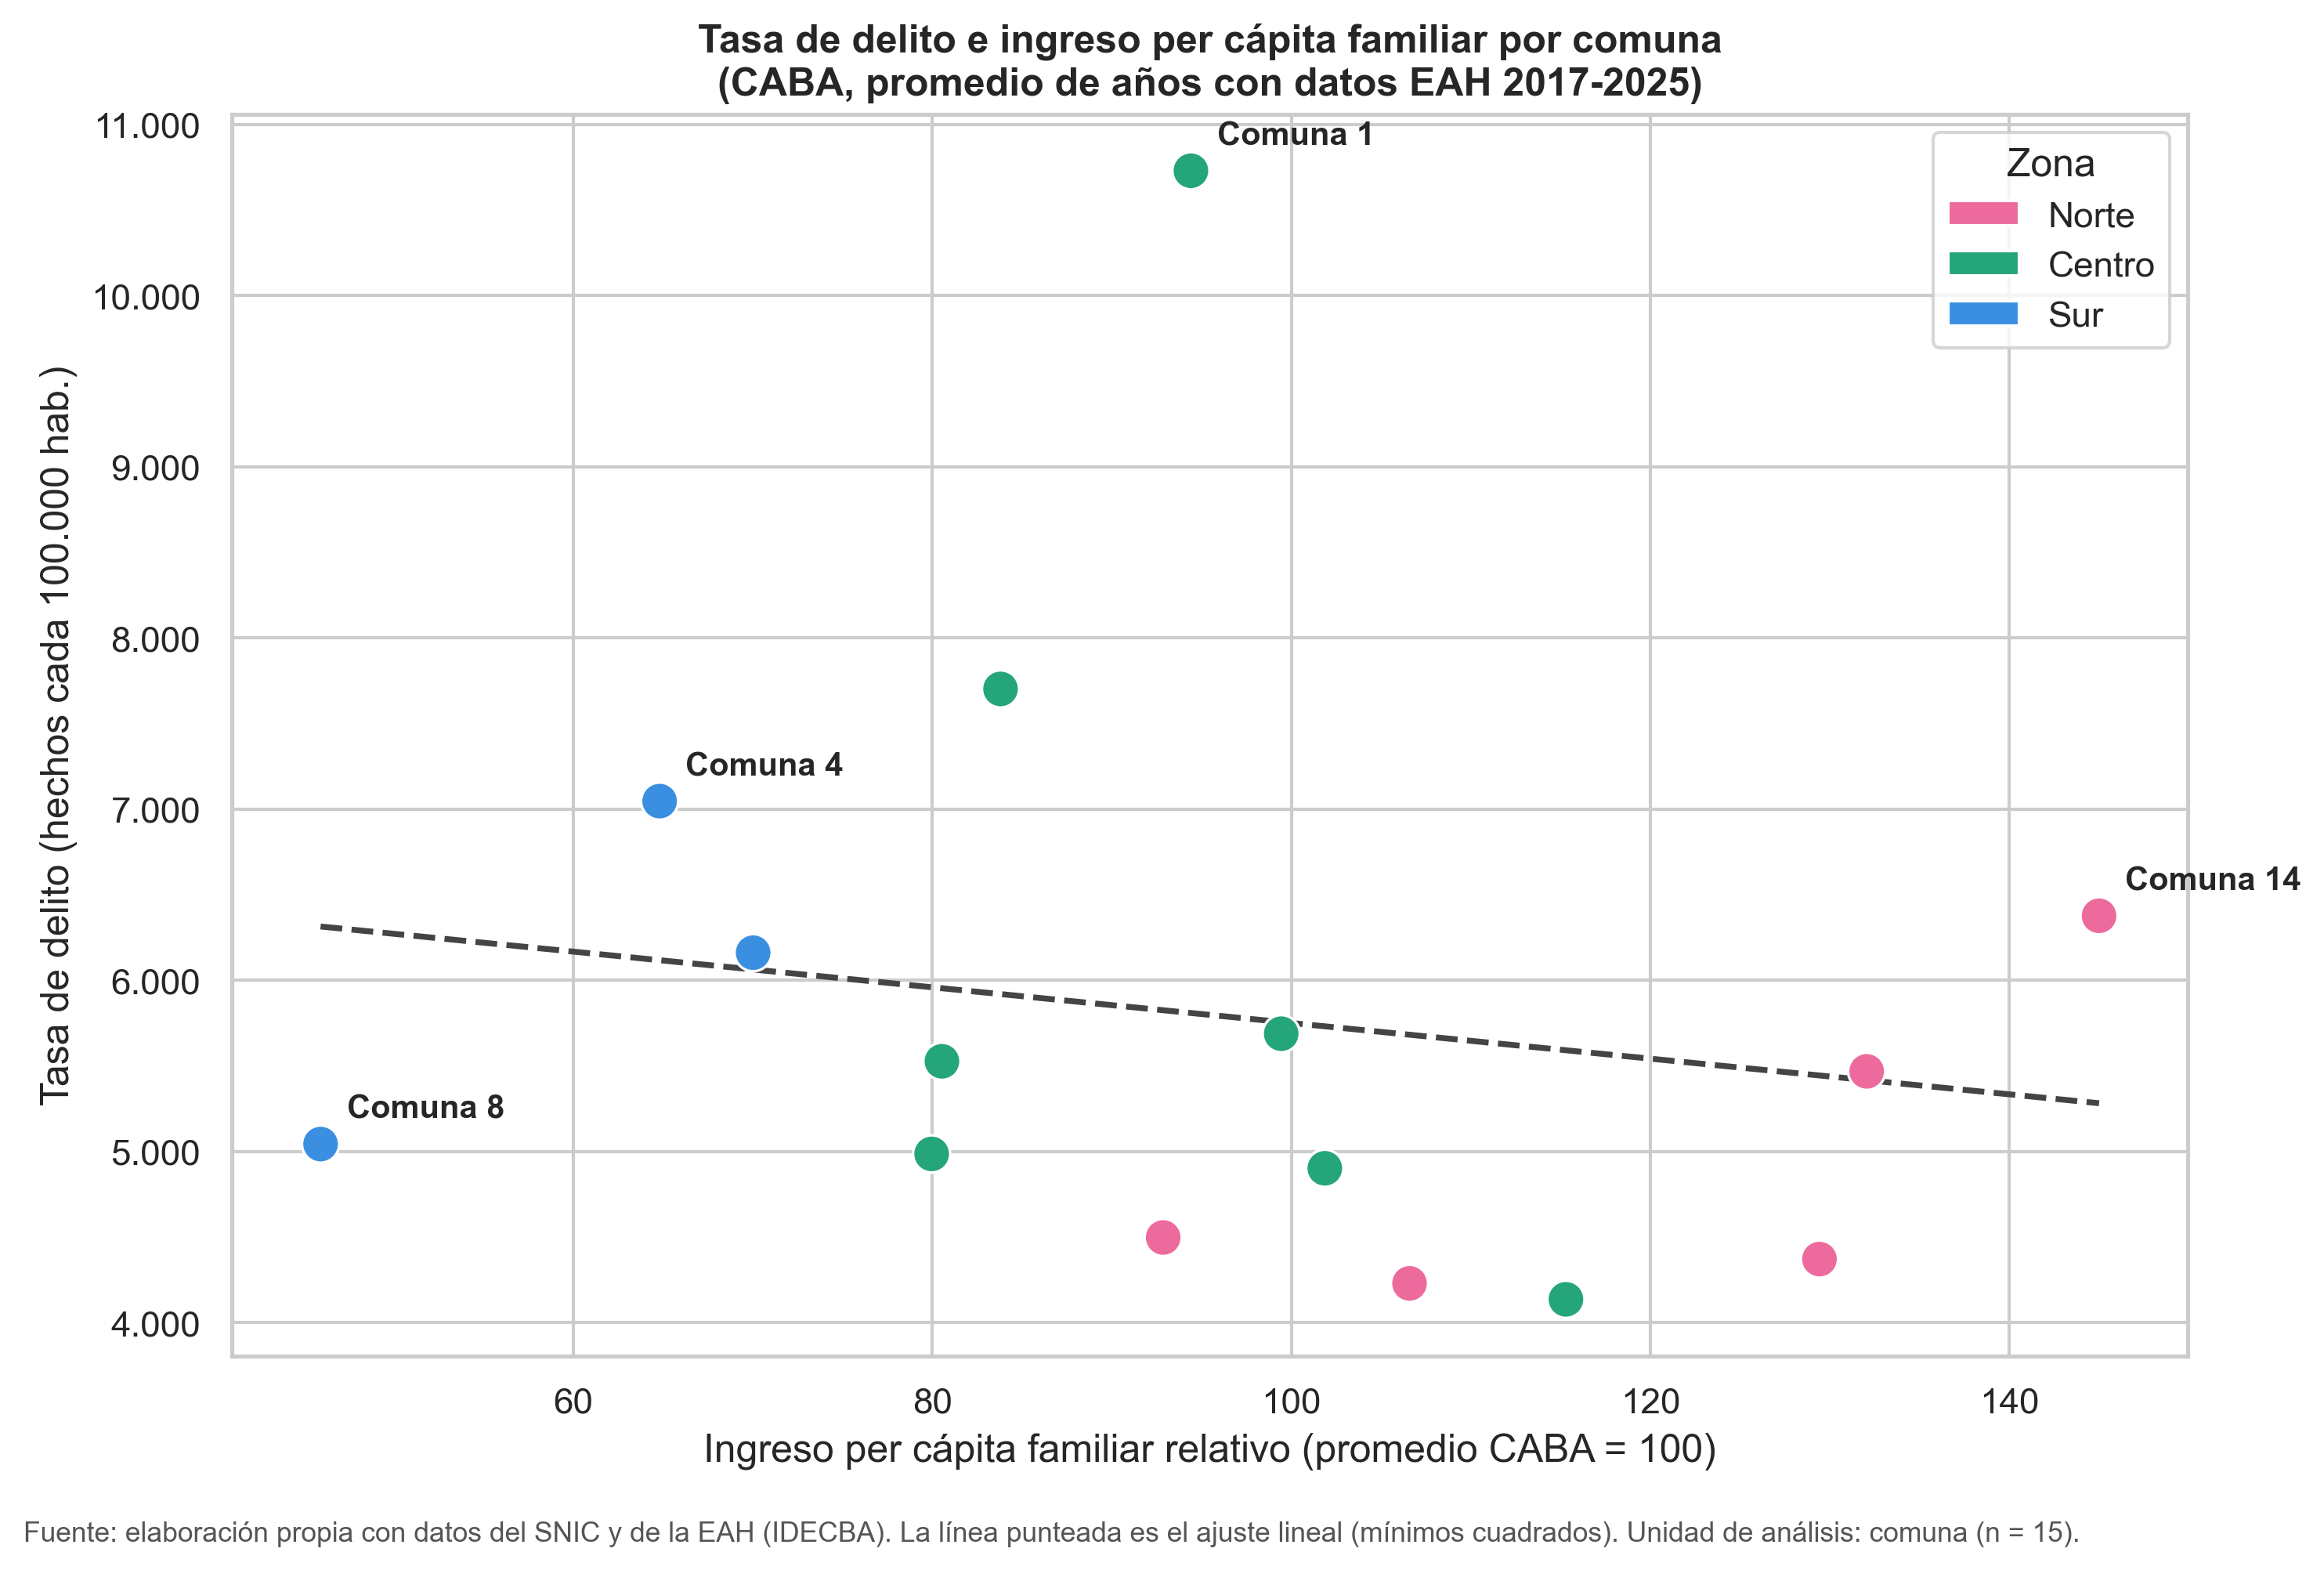
\includegraphics[width=0.66\textwidth]{grafico_a_delito_vs_ingreso.png}
\caption{Tasa de delito e ingreso per cápita familiar relativo por comuna (promedio de los años con datos, 2017--2025). Fuente: SNIC y EAH (IDECBA).}
\label{fig:ingreso}
\end{figure}

Las condiciones territoriales empeoran de norte a sur (Tabla~\ref{tab:zonas}). El Sur concentra los menores ingresos, la mayor desocupación, la menor cobertura de salud, la mayoría de los barrios populares y la mayor proporción de locales vacíos, mientras que el Centro reúne la mayor densidad comercial. Sin embargo, la tasa total de delito no sigue ese orden: el Centro supera al Sur.

\begin{table}[H]
\centering
\small
\caption{Indicadores promedio por zona de la Ciudad.}
\label{tab:zonas}
\begin{tabular}{lrrr}
\toprule
Indicador & Norte & Centro & Sur \\
\midrule
Ingreso per cápita familiar (CABA = 100), EAH 2024 & 118,6 & 95,8 & 67,1 \\
Desocupación (\%), EAH 2024 & 5,0 & 5,4 & 8,7 \\
Población sin obra social (\%), Censo 2022 & 9,4 & 18,5 & 34,4 \\
Barrios populares (promedio por comuna) & 2,4 & 4,7 & 29,0 \\
Locales comerciales cada 1.000 hab. & 25,6 & 33,2 & 23,2 \\
Locales vacíos (\%) & 13,9 & 17,7 & 24,5 \\
\midrule
Tasa de delito total (c/100.000 hab.), SNIC 2017--2025 & 4.815 & 6.049 & 5.952 \\
Robos y hurtos (c/100.000 hab.) & 3.233 & 3.895 & 3.464 \\
Delitos violentos (\% del total) & 12,3 & 14,7 & 21,6 \\
\bottomrule
\end{tabular}
\end{table}

La separación por tipo de delito permite explicar esta diferencia (Figura~\ref{fig:tipo_comuna}). Los robos y hurtos se concentran en las comunas 1 y 3, principales polos comerciales y de circulación de la Ciudad (6.451 y 4.895 hechos cada 100.000 habitantes). En cambio, el peso de los delitos violentos crece de norte a sur: la Comuna 8 encabeza ese ranking (25,9\,\%), seguida por la 4 (21,9\,\%) y la 9 (17,1\,\%), mientras que las comunas 14, 13 y 2 registran los valores más bajos (entre 10,0\,\% y 11,0\,\%).

\begin{figure}[H]
\centering
\begin{minipage}{0.49\textwidth}
\centering
\includegraphics[width=\textwidth]{grafico_robos_hurtos.png}
\end{minipage}\hfill
\begin{minipage}{0.49\textwidth}
\centering
\includegraphics[width=\textwidth]{grafico_delitos_violentos.png}
\end{minipage}
\caption{Robos y hurtos cada 100.000 habitantes (izquierda) y peso de los delitos violentos sobre el total (derecha) por comuna, promedio 2017--2025. Fuente: SNIC.}
\label{fig:tipo_comuna}
\end{figure}

El caso de la Comuna 8 resume este hallazgo: tiene una tasa total por debajo del promedio porque registra pocos robos y hurtos (2.701, un 25\,\% menos que el promedio de las comunas), pero sus delitos violentos (943) superan en un 45\,\% al promedio y son los terceros más altos de la Ciudad.

En cuanto a las hipótesis, la de \textbf{vulnerabilidad} se confirma: es la relación más clara del trabajo. La de \textbf{oportunidad} se confirma parcialmente, ya que el Centro encabeza tanto la densidad comercial como los robos, aunque hay excepciones (la Comuna 10 tiene mucho comercio y pocos robos, y la 14 muchos robos con un nivel comercial medio). La de \textbf{deterioro} también se confirma parcialmente: la Comuna 4 combina la mayor proporción de locales vacíos (29,3\,\%) con un alto peso de delitos violentos, pero los locales vacíos se concentran en las mismas comunas vulnerables, por lo que no es posible separar ambos efectos.

% ---------------------------------------------------------------
% 5. Conclusiones
% ---------------------------------------------------------------
\section{Conclusiones}
CABA presenta una tasa de delitos que duplica la del Conurbano, aunque este registra más hechos en total y mostró un mayor crecimiento entre 2017 y 2025. Los dos territorios también se diferencian en el tipo de delito: en la Ciudad predominan los delitos contra la propiedad y en el Conurbano tienen más peso los delitos contra las personas.

Dentro de CABA, las condiciones socioeconómicas y territoriales no determinan \textbf{cuánto} delito se registra en cada comuna, sino \textbf{qué tipo} de delito predomina. La oportunidad, asociada al comercio y a la circulación de personas, explica dónde se concentran los robos y hurtos; la vulnerabilidad social explica dónde pesan más los delitos violentos.

Los resultados deben leerse con cautela. Se refieren a comunas y no a personas, por lo que no permiten afirmar que los residentes de una comuna con peores condiciones delinquen más o son más victimizados (falacia ecológica). Tampoco demuestran causalidad, ya que hay factores no medidos (población flotante, propensión a denunciar, patrullaje) y el análisis se basa en solo 15 comunas. Se trata de delitos denunciados, sujetos a la cifra negra, y las fuentes corresponden a distintos años (Censo 2022, EAH 2024 y SNIC 2017--2025). Como extensiones posibles se proponen incorporar datos de victimización, que capturan los delitos no denunciados, y replicar el análisis territorial en los partidos del Conurbano.

% ---------------------------------------------------------------
% 6. Reflexión metodológica
% ---------------------------------------------------------------
\section{Reflexión metodológica}
Se utilizó Claude (Anthropic) como asistente en todas las etapas: para revisar la estructura del notebook frente a las pautas, decidir el tratamiento de nulos y tipos de delito, escribir y adaptar el código de los gráficos, integrar las distintas partes del análisis y redactar borradores de las interpretaciones y de este informe. El detalle de su uso por sección, con ejemplos de las instrucciones empleadas, figura en el notebook. Todas las cifras propuestas se contrastaron con las salidas del código y cada integrante leyó el informe de forma independiente para controlar que las afirmaciones coincidieran con el notebook y los datos originales. Entre los aprendizajes se destacan la importancia de documentar las exclusiones de datos, de unificar criterios (zonas, colores y nombres de variables) al integrar el trabajo de distintos integrantes y de distinguir entre la cantidad y el tipo de delito.

% ---------------------------------------------------------------
% 7. Bibliografía
% ---------------------------------------------------------------
\begin{thebibliography}{9}
\small
\bibitem{snic} Ministerio de Seguridad de la Nación. \textit{Sistema Nacional de Información Criminal (SNIC) -- Departamentos. Anual. Años 2000--2025}. \url{https://www.argentina.gob.ar/seguridad/estadisticascriminales/bases-de-datos}
\bibitem{eah} Instituto de Estadística y Censos de la Ciudad de Buenos Aires (IDECBA). \textit{Encuesta Anual de Hogares}. \url{https://www.estadisticaciudad.gob.ar}
\bibitem{censo} INDEC. \textit{Censo Nacional de Población, Hogares y Viviendas 2022. Resultados definitivos}. \url{https://www.indec.gob.ar/indec/web/Nivel4-Tema-2-41-165}
\bibitem{bp} Gobierno de la Ciudad de Buenos Aires. \textit{Barrios populares}. BA Data. \url{https://data.buenosaires.gob.ar/dataset/barrios-populares}
\bibitem{usos} Gobierno de la Ciudad de Buenos Aires. \textit{Relevamiento de Usos del Suelo 2022--2024}. BA Data. \url{https://data.buenosaires.gob.ar/dataset/relevamiento-usos-suelo}
\end{thebibliography}

\end{document}
